\section{Enablers}
\label{sec:enables}


\subsection{}
% Collaborative Analysis Framework

% By leveraging a state-of-the-art memory analysis framework, we are able to
% disprove more dependences to allow less or inexpensive speculations.


% Enabler Introduction

In this work, we introduce a set of transformations to explore more
opportunities of parallelization. We call these enabling transformations
Enablers.

%  How to query Enabler?

One thing that hinders these Enablers from working in a coordinated way is
the phase-ordering problem, which means one transformation could be disabled
by a previous transformation. Another problem is the increasing
implementation and maintainance difficulty when more and more Enablers are
put in the framework. To avoid these problems, we carefully organize the
framework in a way that all Enablers are modular and independent. As a first
step, all loop-carried dependences are identified by the frontend and passed
to each Enabler, who tries to address each dependence by its best effort and
returns a remedy along with the cost if a way to remove the dependence is
available. If all dependences are removable by at least one Enablers, the
parallel code generation part will choose the remedy with the lowest cost
for each dependence and generate the parallel binary. This scheme seperates
the desicion part from the actual transformation and allows us to evaluate
the cost of each dependence separetely and choose the most profitable plan
instead of applying all transformations in a fixed order. For simplicity, we
assigned to each Enabler a predefined cost in this work. Yet in Table.
\ref{table:enabler-stats}, we provided the statistics of the applicable and
chosen Enabler to show how this framework makes the tradeoff when more than
one Enablers are available. This study is not available for a traditional
approach of transformations.

The analysis passes and the transformation passes are seperated. Even though
it has been suggested before, in this work, we have a smaller set of
Enablers with stronger capability.

% Enabler Description
\subsection{Enabler Description}

Non Speculative Enablers

\begin{itemize}
    \item Conservative Reduction (ReduxRemed)
        % Both scalar and memory reduction

    \item Conservative Privatization (PrivRemed)
        % Removes loop-carried false memory dependences on conservatively provable privitizable objects

    \item Memory Versioning (MemVerRemed)
        % Assumes privatized memory for each thread
        % Removes loop-carried false memory dependences
        % Stronger but more expensive than PrivRemed
        % Process-based parallelization enforces this remediator

    \item Counted Loop Detection (CountedIVRemed)
        % Removes loop-carried register and control dependences related to induction variables on counted loops

    \item TXIO (TXIORemed)
        % I/O deferral
        % Delays execution of instructions with side-effects, such as I/O operations

    \item Conservative Loop Fission (LoopFissionRemed)
        % Separate non-DOALL SCCs to an initial sequential stage (loop in this case)
        % Only small sequential stages considered
        % No usage of speculative remediators to achieve separation
\end{itemize}

Speculative Enablers

\begin{itemize}
    \item Control Speculation (ControlSpecRemed)
        % Based on edge profile info, removes control flow edges and considers all basic blocks dominated by these edges as speculatively dead
        % Inexpensive runtime validation

    \item Value Prediction (LoadedValuePred)
        % Some load instructions always read a single, predictable value from memory
        % Loop-Invariant Loaded-Value
        % Inexpensive runtime validation

    \item Header-phi prediction (HeaderPhiPredRemed)
        % Some phi instructions have a predictable value.
        % Allows removal of loop-carried register dependeces
        % Inexpensive runtime validation

    \item Separation Speculation (LocalityRemed)

        % Johnson et al. PLDI '12

        % Separation speculation partitions a program's allocations into a few disjoint "families" of objects and speculatively assumes that every pointer in the program refers exclusively to objects in one family. Under this assumption, if two pointers reference distinct families, they cannot alias.

        % Relatively inexpensive runtime validation due to small number of families, allocation of objects in family-specific memory regions, runtime optimizations and thread-local checks (no communication among concurrent threads needed).

        % Secondary speculation built on top of separation speculation:

        %     Read-only speculation
        %         Read-only family
        %         Some memory objects are never modified but static dependence analysis is sometimes unable to prove this property
        %         Objects in the read-only family are only accessed by read-only memory operations. Thus, speculatively read-only memory operations never experience flow, anti or output dependences
        %         Apart from separation speculation validation, no other validation is required

        %     Speculative accumulator expansion
        %         Compiler identifies accumulators as values which are repeatedly updated with an associative and commutative operator (a reduction) but whose intermediate values are otherwise unused within the loop. Static dependence sometimes fails to prove that every access to a given storage location is a reduction or that intermediate values are never used.
        %         The pointer-family assumption establishes that objects in the reduction family are only accessed by load-reduce-store sequences and consequently that intermediate values cannot be otherwise observed or modified.
        %         Apart from separation speculation validation, no other validation is required

        %     Speculative privatization
        %         Reuse of data structures with no flow dependences from one iteration to the other prevents parallelization due to anti or output dependences.
        %         Addressed by having a private copy of the data structure for each iteration
        %         Assumption: loads from certain private objects never read values stored during earlier iterations of the loop.
        %         Privatization criteria validated in two phases, one thread-local and one more expensive that requires communication among threads.

        %     Object-lifetime speculation
        %         Short-lived objects
        %         Some objects allocated within a loop iteration are always deallocated before the end of that same iteration. Static dependence analysis often fails to identify this case.
        %         Loads from or stores to such objects cannot depend on memory accesses in other iterations.
        %         Extra validation on top of separation speculation validation: object lifetime speculation must validate that short-lived objects never outlive their iteration. Thread-local checks.

    \item Memory Flow Speculation (SmtxSlampRemed & SmtxLampRemed)
        % Assumes the absence of flow dependences between memory operations when not manifested during profiling.
        % Provides as much or more an enabling effect than many other types of speculation.
        % Expensive validation. Requires communication among concurrent threads.

    \item Speculative AA stack (MemSpecAARemed)
        % Allows collaboration among memory flow speculation, control speculation, value prediction, speculative points-to analysis and static analysis.
        % Demonstrates the power of collaboration among remediators, and between speculation techniques and static analysis.
        % Provides at least as much coverage as all the remediators addressing mem deps combined (only excludes SLAMP mem spec and localityaa).

    \item Speculative Loop Fission (LoopFissionRemed)
        % Same as Conservative Loop Fission apart from the fact that it requires usage of speculative remediators to achieve separation

    \item Pointer-Residue Speculation (PtrResidueRemed)
        % Never part of a paper. Never evaluated. Idea published in Nick Johnson's thesis
        % Separation speculation disambiguates references to different objects, but does not disambiguate references within the same object. Pointer-residue speculation works at the sub-object level.
        % It disambiguates different fields within an object and in some cases recognizes different regular strides across an array.
        % It characterizes each pointer expression in the program according to the possible values of its four least-significant bits (residue).
        % Examines whether residue sets are disjoint with respect to the size of the memory accesses of two given operations.
\end{itemize}

Second Level Enabler
\begin{itemize}
    \item Replicable Stage (RepStageRemedy)
\end{itemize}

\subsection{Enabler Statistics}
% Insert the table here

% 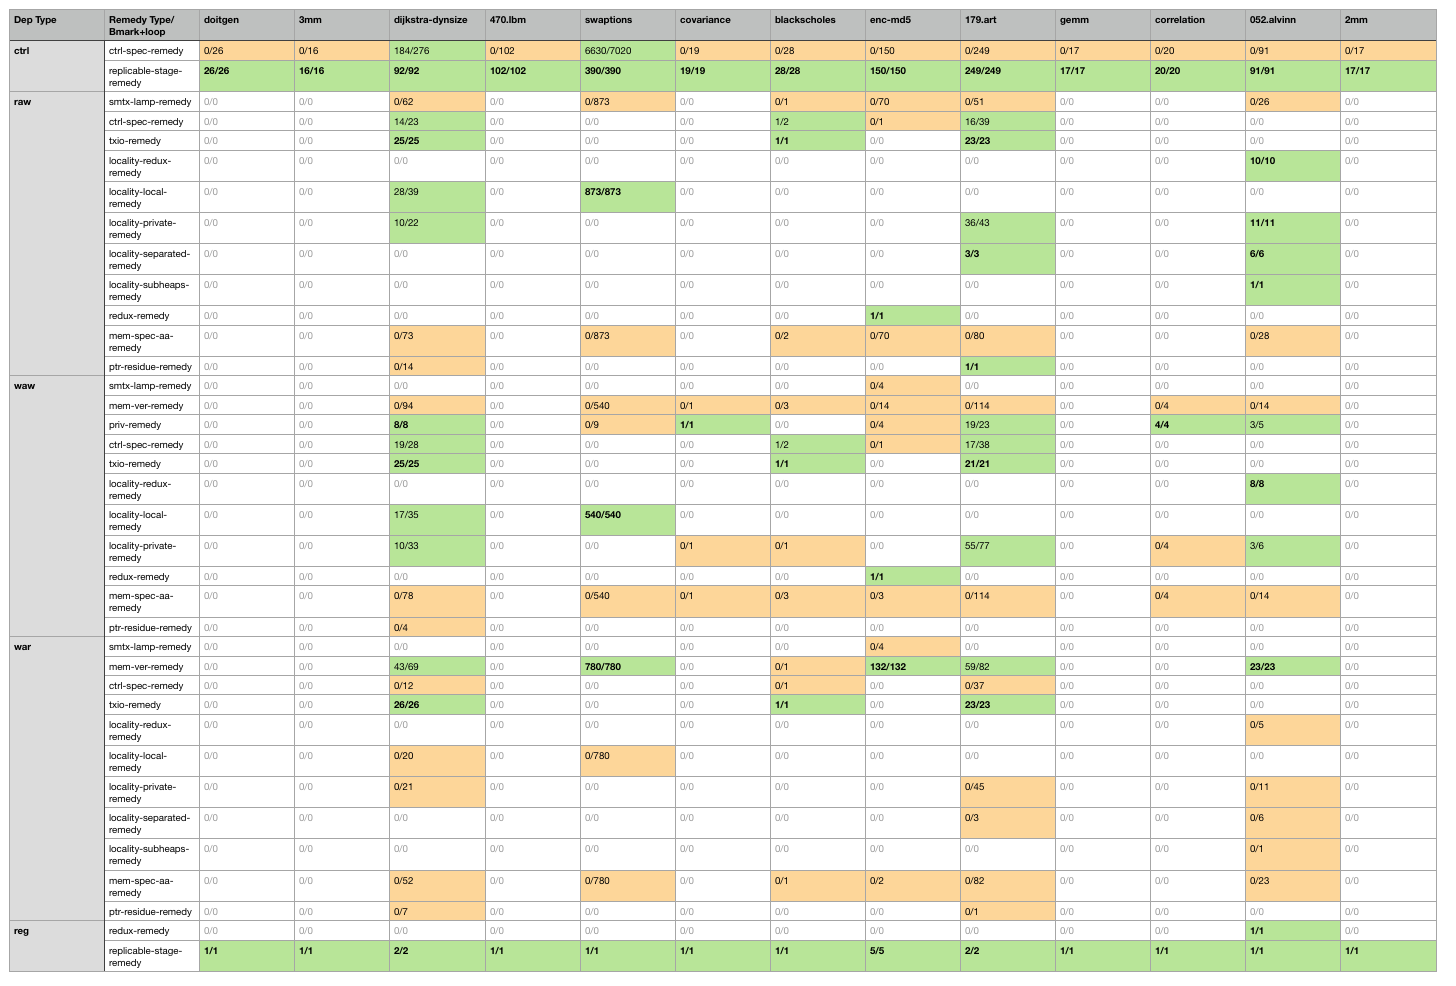
\includegraphics[width=\textwidth]{figures/table.png}
% \label{table:enabler-stats}


% \begin{table}[]
% \label{table:enabler-stats}
% \begin{tabular}{lllllllllllllll}

% Dep Type & Remedy Type/Bmark+loop    & doitgen & 3mm   & dijkstra-dynsize &
% 470.lbm & swaptions & covariance & blackscholes & enc-md5 & 179.art & gemm  &
% correlation & 052.alvinn & 2mm   \\

% ctrl     & ctrl-spec-remedy          & 0/26    & 0/16  & 184/276          &
% 0/102   & 6630/7020 & 0/19       & 0/28         & 0/150   & 0/249   & 0/17  &
% 0/20        & 0/91       & 0/17  \\

%          & replicable-stage-remedy   & 26/26   & 16/16 & 92/92            &
%          102/102 & 390/390   & 19/19      & 28/28        & 150/150 & 249/249 &
%          17/17 & 20/20       & 91/91      & 17/17 \\

% raw      & smtx-lamp-remedy          & 0/0     & 0/0   & 0/62             & 0/0
% & 0/873     & 0/0        & 0/1          & 0/70    & 0/51    & 0/0   & 0/0
% & 0/26       & 0/0   \\
%          & ctrl-spec-remedy          & 0/0     & 0/0   & 14/23            & 0/0
%          & 0/0       & 0/0        & 1/2          & 0/1     & 16/39   & 0/0   &
%          0/0         & 0/0        & 0/0   \\

%          & txio-remedy               & 0/0     & 0/0   & 25/25            & 0/0
%          & 0/0       & 0/0        & 1/1          & 0/0     & 23/23   & 0/0   &
%          0/0         & 0/0        & 0/0   \\

%          & locality-redux-remedy     & 0/0     & 0/0   & 0/0              & 0/0
%          & 0/0       & 0/0        & 0/0          & 0/0     & 0/0     & 0/0   &
%          0/0         & 10/10      & 0/0   \\

%          & locality-local-remedy     & 0/0     & 0/0   & 28/39            & 0/0
%          & 873/873   & 0/0        & 0/0          & 0/0     & 0/0     & 0/0   &
%          0/0         & 0/0        & 0/0   \\

%          & locality-private-remedy   & 0/0     & 0/0   & 10/22            & 0/0
%          & 0/0       & 0/0        & 0/0          & 0/0     & 36/43   & 0/0   &
%          0/0         & 11/11      & 0/0   \\

%          & locality-separated-remedy & 0/0     & 0/0   & 0/0              & 0/0
%          & 0/0       & 0/0        & 0/0          & 0/0     & 3/3     & 0/0   &
%          0/0         & 6/6        & 0/0   \\

%          & locality-subheaps-remedy  & 0/0     & 0/0   & 0/0              & 0/0
%          & 0/0       & 0/0        & 0/0          & 0/0     & 0/0     & 0/0   &
%          0/0         & 1/1        & 0/0   \\

%          & redux-remedy              & 0/0     & 0/0   & 0/0              & 0/0
%          & 0/0       & 0/0        & 0/0          & 1/1     & 0/0     & 0/0   &
%          0/0         & 0/0        & 0/0   \\

%          & mem-spec-aa-remedy        & 0/0     & 0/0   & 0/73             & 0/0
%          & 0/873     & 0/0        & 0/2          & 0/70    & 0/80    & 0/0   &
%          0/0         & 0/28       & 0/0   \\

%          & ptr-residue-remedy        & 0/0     & 0/0   & 0/14             & 0/0
%          & 0/0       & 0/0        & 0/0          & 0/0     & 1/1     & 0/0   &
%          0/0         & 0/0        & 0/0   \\

% waw      & smtx-lamp-remedy          & 0/0     & 0/0   & 0/0              & 0/0
% & 0/0       & 0/0        & 0/0          & 0/4     & 0/0     & 0/0   & 0/0
% & 0/0        & 0/0   \\

%          & mem-ver-remedy            & 0/0     & 0/0   & 0/94             & 0/0
%          & 0/540     & 0/1        & 0/3          & 0/14    & 0/114   & 0/0   &
%          0/4         & 0/14       & 0/0   \\

%          & priv-remedy               & 0/0     & 0/0   & 8/8              & 0/0
%          & 0/9       & 1/1        & 0/0          & 0/4     & 19/23   & 0/0   &
%          4/4         & 3/5        & 0/0   \\

%          & ctrl-spec-remedy          & 0/0     & 0/0   & 19/28            & 0/0
%          & 0/0       & 0/0        & 1/2          & 0/1     & 17/38   & 0/0   &
%          0/0         & 0/0        & 0/0   \\

%          & txio-remedy               & 0/0     & 0/0   & 25/25            & 0/0
%          & 0/0       & 0/0        & 1/1          & 0/0     & 21/21   & 0/0   &
%          0/0         & 0/0        & 0/0   \\

%          & locality-redux-remedy     & 0/0     & 0/0   & 0/0              & 0/0
%          & 0/0       & 0/0        & 0/0          & 0/0     & 0/0     & 0/0   &
%          0/0         & 8/8        & 0/0   \\

%          & locality-local-remedy     & 0/0     & 0/0   & 17/35            & 0/0
%          & 540/540   & 0/0        & 0/0          & 0/0     & 0/0     & 0/0   &
%          0/0         & 0/0        & 0/0   \\

%          & locality-private-remedy   & 0/0     & 0/0   & 10/33            & 0/0
%          & 0/0       & 0/1        & 0/1          & 0/0     & 55/77   & 0/0   &
%          0/4         & 3/6        & 0/0   \\

%          & redux-remedy              & 0/0     & 0/0   & 0/0              & 0/0
%          & 0/0       & 0/0        & 0/0          & 1/1     & 0/0     & 0/0   &
%          0/0         & 0/0        & 0/0   \\

%          & mem-spec-aa-remedy        & 0/0     & 0/0   & 0/78             & 0/0
%          & 0/540     & 0/1        & 0/3          & 0/3     & 0/114   & 0/0   &
%          0/4         & 0/14       & 0/0   \\

%          & ptr-residue-remedy        & 0/0     & 0/0   & 0/4              & 0/0
%          & 0/0       & 0/0        & 0/0          & 0/0     & 0/0     & 0/0   &
%          0/0         & 0/0        & 0/0   \\

% war      & smtx-lamp-remedy          & 0/0     & 0/0   & 0/0              & 0/0
% & 0/0       & 0/0        & 0/0          & 0/4     & 0/0     & 0/0   & 0/0
% & 0/0        & 0/0   \\

%          & mem-ver-remedy            & 0/0     & 0/0   & 43/69            & 0/0
%          & 780/780   & 0/0        & 0/1          & 132/132 & 59/82   & 0/0   &
%          0/0         & 23/23      & 0/0   \\

%          & ctrl-spec-remedy          & 0/0     & 0/0   & 0/12             & 0/0
%          & 0/0       & 0/0        & 0/1          & 0/0     & 0/37    & 0/0   &
%          0/0         & 0/0        & 0/0   \\

%          & txio-remedy               & 0/0     & 0/0   & 26/26            & 0/0
%          & 0/0       & 0/0        & 1/1          & 0/0     & 23/23   & 0/0   &
%          0/0         & 0/0        & 0/0   \\

%          & locality-redux-remedy     & 0/0     & 0/0   & 0/0              & 0/0
%          & 0/0       & 0/0        & 0/0          & 0/0     & 0/0     & 0/0   &
%          0/0         & 0/5        & 0/0   \\

%          & locality-local-remedy     & 0/0     & 0/0   & 0/20             & 0/0
%          & 0/780     & 0/0        & 0/0          & 0/0     & 0/0     & 0/0   &
%          0/0         & 0/0        & 0/0   \\

%          & locality-private-remedy   & 0/0     & 0/0   & 0/21             & 0/0
%          & 0/0       & 0/0        & 0/0          & 0/0     & 0/45    & 0/0   &
%          0/0         & 0/11       & 0/0   \\

%          & locality-separated-remedy & 0/0     & 0/0   & 0/0              & 0/0
%          & 0/0       & 0/0        & 0/0          & 0/0     & 0/3     & 0/0   &
%          0/0         & 0/6        & 0/0   \\

%          & locality-subheaps-remedy  & 0/0     & 0/0   & 0/0              & 0/0
%          & 0/0       & 0/0        & 0/0          & 0/0     & 0/0     & 0/0   &
%          0/0         & 0/1        & 0/0   \\

%          & mem-spec-aa-remedy        & 0/0     & 0/0   & 0/52             & 0/0
%          & 0/780     & 0/0        & 0/1          & 0/2     & 0/82    & 0/0   &
%          0/0         & 0/23       & 0/0   \\

%          & ptr-residue-remedy        & 0/0     & 0/0   & 0/7              & 0/0
%          & 0/0       & 0/0        & 0/0          & 0/0     & 0/1     & 0/0   &
%          0/0         & 0/0        & 0/0   \\

% reg      & redux-remedy              & 0/0     & 0/0   & 0/0              & 0/0
% & 0/0       & 0/0        & 0/0          & 0/0     & 0/0     & 0/0   & 0/0
% & 1/1        & 0/0   \\

%          & replicable-stage-remedy   & 1/1     & 1/1   & 2/2              & 1/1
%          & 1/1       & 1/1        & 1/1          & 5/5     & 2/2     & 1/1   &
%          1/1         & 1/1        & 1/1
% \end{tabular}
% \end{table}

% Discussion of the table


% Discuss about LLVM
\subsection{LLVM Related Issues}

To make best use of LLVM, we have to let it generate the simplest
intermediate representation (IR) without introducing optimizations that
might disable any Enabler of this framework. We carefully selected a set of
LLVM optimizations and added some other modifications to generate a proper
IR to work on.

Other modifications:

\begin{itemize}
\item Optimization Level

% For example?
LLVM optimization passes are important to simplify the IR however some of
them are destructive to parallelization. The previous approach was using no
optimization to generate the first IR and then applying a selected set of
LLVM passes to optmize the code. However, we noticed that when no
optimization is used in the frontend (\textit{clang -O0 -Xclang
-disable-O0-optnone}), some LLVM intrinsics which can be helpful to the
framework are lost. For example, for stack variables that are allocated in
an inner loop, LLVM should move the \textit{alloca} to the function header
and provide a pair of lifetime start/end intrinsics. The lifetime intrinsic
does not come with no optimization. To get around this, we chose
optimization level 1 for only Clang frontend optimizations and disabled LLVM
Opt passes (\textit{-O1 -Xclang -disable-llvm-passes}). This gives us the
intended behavior.


\item PHI Node

PHI nodes introduce more complicated data flow. LLVM will sink some
duplicated instructions into PHI nodes and create extra hassle for our
system to identify loop-carried data and create separation for different
objects. We disabled several options in LLVM passes to inhibit this
behavior.

\item Inlining

Inlining is a huge deal for parallelizing programs. For sequential program,
the inlining optimization is needed when the cost of calling a function is
big. The tradeoff is between speed and code size. Large functions that are
called multiple times are usually not inlined. However, for parallelization,
inlining can help us differenciate callsites and improve the accuracy of
both static analysis and memory profiling. In this work, we adopted an
aggresive approach of inlining with which most functions in the hot loops
are inlined. The tradeoff here is mainly between the accuracy and the
complexity (speed) of analysis. To reduce the complexity and improve the
speed, we identified functions that are not called in profile runs and
skipped inlining for them because they can be speculated away.

\end{itemize}
